% Nallino, Part I p. 265: Schiaparelli's figure of the second solution for the distance of the Moon,
% redrawn from the print: the semicircle AZB about E, the Earth through F, the vertical EZ, the lines
% FL and EL, the perpendicular FQ (dashed), the dotted arc of the angle z, and the letters.
% Measured on the scan (_intake/latin/tools/fig265).
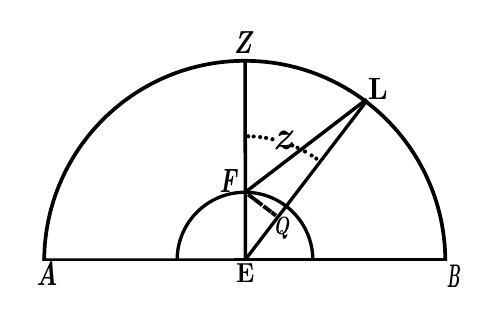
\begin{tikzpicture}[x=0.9964pt,y=-0.9964pt,line cap=butt,every node/.style={font=\fontsize{11}{11}\bfseries\itshape\selectfont,inner sep=0pt}]
\useasboundingbox (0,0) rectangle (159.00,96.00);
\draw[line width=0.94pt] (5.32,84.11) -- (152.14,84.07);  % the diameter AB
\draw[line width=1.27pt] (78.96,84.09) -- (78.86,12.01);  % the vertical EZ
\draw[line width=1.25pt] (78.92,59.68) -- (122.94,25.97);  % the line FL
\draw[line width=1.19pt] (78.96,84.09) -- (123.12,26.33);  % the line EL
\draw[line width=1.34pt] (5.99,84.12) arc[start angle=-179.50,end angle=-0.54,radius=72.74];
\draw[line width=1.20pt] (54.20,84.10) arc[start angle=-179.55,end angle=-0.48,radius=24.61];
\fill (80.00,39.37) circle[radius=0.75];  % a dot of the arc of the angle z at -88.67 deg
\fill (81.97,39.46) circle[radius=0.75];  % a dot of the arc of the angle z at -86.14 deg
\fill (84.32,39.68) circle[radius=0.75];  % a dot of the arc of the angle z at -83.11 deg
\fill (86.44,39.99) circle[radius=0.75];  % a dot of the arc of the angle z at -80.37 deg
\fill (88.78,40.45) circle[radius=0.75];  % a dot of the arc of the angle z at -77.32 deg
\fill (95.99,42.73) circle[radius=0.75];  % a dot of the arc of the angle z at -67.62 deg
\fill (97.85,43.54) circle[radius=0.75];  % a dot of the arc of the angle z at -65.02 deg
\fill (100.58,44.93) circle[radius=0.75];  % a dot of the arc of the angle z at -61.09 deg
\fill (102.96,46.34) circle[radius=0.75];  % a dot of the arc of the angle z at -57.55 deg
\fill (104.69,47.50) circle[radius=0.75];  % a dot of the arc of the angle z at -54.89 deg
% the dashed perpendicular FQ on EL
\draw[line width=1.39pt] (79.96,60.47)--(82.12,62.11) (82.23,62.20)--(85.09,64.38) (85.51,64.70)--(88.26,66.80) (88.45,66.94)--(90.05,68.16);
\node at (77.92,5.46) {\normalfont\fontsize{11}{11}\bfseries\itshape\selectfont \resizebox{6.51pt}{7.89pt}{Z}};
\node at (127.01,22.04) {\normalfont\fontsize{11}{11}\bfseries\selectfont \resizebox{7.22pt}{7.63pt}{L}};
\node at (92.39,40.92) {\normalfont\fontsize{11}{11}\bfseries\itshape\selectfont \resizebox{6.72pt}{6.60pt}{z}};
\node at (72.64,55.50) {\normalfont\fontsize{11}{11}\bfseries\itshape\selectfont \resizebox{6.16pt}{8.36pt}{F}};
\node at (91.99,72.84) {\normalfont\fontsize{11}{11}\bfseries\itshape\selectfont \resizebox{5.71pt}{6.19pt}{Q}};
\node at (7.03,89.34) {\normalfont\fontsize{11}{11}\bfseries\itshape\selectfont \resizebox{7.83pt}{8.34pt}{A}};
\node at (78.96,89.16) {\normalfont\fontsize{11}{11}\bfseries\selectfont \resizebox{6.62pt}{6.82pt}{E}};
\node at (154.30,89.98) {\normalfont\fontsize{11}{11}\bfseries\itshape\selectfont \resizebox{4.78pt}{8.11pt}{B}};
\end{tikzpicture}
